
\chapter{Probabilistic Graphical Models}

\section{Probabilitic Inference}

Suppose having a set of random variates (either discrete or continuous) $x = (x_1,\dots, x_n), z = (z_1,\dots, z_m)$ with joint probability distribution $p(x,z)$.

To reason about such a model, we would perform:
\begin{itemize}
    \item \textbf{Marginalization}: $p(x) = \sum_z p(x,z) = \int p(x,z)\,dz\,dx_{-i}$
    \item \textbf{Conditioning}: $p(x|z) = \frac{p(x,z)}{p(z)}$
\end{itemize}

These operations can be combined to perform \textbf{inference} on the model, i.e. to compute the probability of some variables given the values of others.

\[
    p(z_j|x_i = \bar{x}_i) = \frac{p(\bar{x_i}), z_j}{p(\bar{x}_i)} = \frac{\sum_{\bar{z}_j} p(\bar{x}_i, \bar{z}_j)}{p(\bar{x}_i)} = \frac{\int p(x,z)\,dx_{-i}\,dz_{j}}{\int P(x,z)\,dx_{-i}\,dz}
\]

What is the cost of computation of performing these operations?

Well, focusing on discrete values for $z$ such that $z_i \in {0,1}$ and considering the marginalization over it:
\[
    p(x) = \sum_{z \in Z}^{}p(x,z)
\]

Here $z \in Z, with |Z| = 2^m$, resulting in an asympotically exponential cost in the number of variables.

Let's set up a strategy to perform inference and marginalizaton in a more efficient way. 

\subsection*{Factorisation}

Consider $p(x_1,\dots, x_n)$. Applying the laws of probability we can write
\[
\begin{array}{rl}
    p(x_1,\dots, x_n) &= p(x_1)p(x_2|x_1)p(x_3|x_1,x_2)\dots p(x_n|x_1,\dots, x_{n-1}) \\
    &= \prod_{i=1}^{n} p(x_i|x_1,\dots, x_{i-1}) \\
    &= p(x_n|x_1,\dots, x_{n-1})p(x_{n-1}|x_1,\dots, x_{n-2})\dots p(x_1)
\end{array}
\]

What is then the cost in terms of computer memory to store these three representation of out distribution? Suppose $x_i \in {1, \dots, k}$, we have the following costs:
\begin{itemize}
    \item $p(x_1)$ costs $k-1 = O(k)$ floating point numbers (single or double precision)
    \item $p(x_2|x_1)$ costs $k(k-1) = O(k^2)$ float numbers (we have different distributions for $x_2$, each costing $k-1$ floats)
    \item In general $p(x_n|x_1,\dots, x_{n-1})$ costs $O(k^n)$ float numbers 
    \item Factorization costs $O(k^n)$ float numbers, unfeasible 
\end{itemize}

%\begin{observationblock}[Factorization]
%   given a joint distribution $p(x_1,\dots, \x_n)$, there are several ways ($n!$) of factorizing it, similarly to the one above, depending on the order of the variables. Any of these choices may correspond to a different factorization. The problem of identifying the most parsimoious factorization if known to be NP-hard.
%\end{observationblock}

\textbf{Probabilistic Graphical Models (PGM)} are models of a probability distribution that describe/impose a certain factorization, hence allowing us to store and make inference effectively with joint distributions. There are three main kind of PGM:
\begin{itemize}
    \item Bayesian Networks
    \item Markov Random Fields
    \item Factor Graphs
\end{itemize}

\section{Bayesian Networks}

\begin{definitionblock}[Bayesian Network]
    A Bayesian Network is a directed acyclic graph (DAG) $G = (V,E)$ where:
    \begin{itemize}
        \item $V = \{x_1,\dots, x_n\}$ is a set of random variables
        \item $E \subseteq V \times V$ is a set of directed edges
    \end{itemize}
    such that each node $x_i$ is associated with a conditional probability distribution $p(x_i|pa(x_i))$ where $pa(x_i)$ is the set of parents of $x_i$ in $G$.
\end{definitionblock}

\begin{figure}[H]
    \centering
    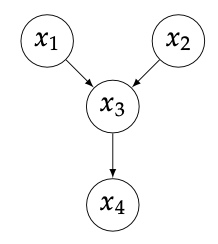
\includegraphics[width=0.4\textwidth]{assets/fig1.png}
\end{figure}

\begin{figure}[H]
    \centering
    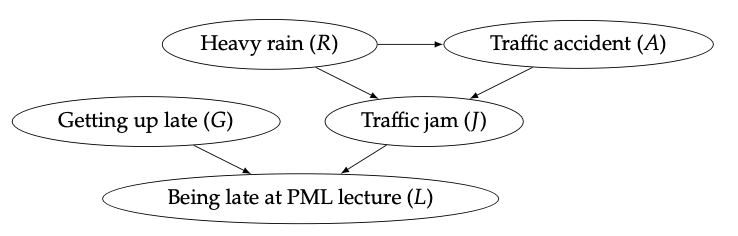
\includegraphics[width=0.8\textwidth]{assets/fig2.png}
    \caption{Example of a Bayesian Network}
\end{figure}

This BN corresponds to the following factorization:
\[
    p(L,G,J,R,A) = p(L|G,J)p(J|R,A)p(A|R)p(R)p(G)
\]

\begin{tipsblock}
    Directed edges does mean causality. BN \textbf{are not} a causal model.
\end{tipsblock}


\subsection*{Notational Conventions}

\begin{itemize}
    \item Observed nodes (Random variables of which we know the value) are \textbf{coloured} or shadowed
    \item Plated nodes are a shorthand for a collection of nodes. 
    \item Deterministic quantities represented as small solid circles. These are fixed parameters of the model (represented graphically as $\dot \alpha$)
\end{itemize}

\begin{exampleblock}[Mixture of Gaussians]
    As an example suppose to have a RV $z$ that follows a discrete distribution and another RV $x$ that is normally distributed with mean $\mu(z)$, depending on the value of $z$, and variance $\sigma^2$. This model is known as a \textbf{mixture of gaussians}.
    
    We can write the joint distribution as:
    \[
        p(x,z) = p(z)p(x|z) = p(z)\mathcal{N}(x|\mu(z), \sigma^2)
    \]

    with $p(x|z) = \mathcal{N}(x|\mu_z, \sigma^2)$

    Typically, in this scenario we have at our disposal $n$ observations of the variable $x$, $\bar{x} = x_1,\dots, x_n$, while the corresponding variable $z$ is unobserved (hence $z$ is a \textbf{latent variable}). We typically want to compute $p(z|\bar{x})$.

    We can have two scenarios here: in the first $\bar{x}$ are sampled from a single realization of the variable $z$, while in the second one each $x_i$ may have been drawn with a different $z_i$, hence we are interested in computing $p(z_i!x_i)$:

    \begin{figure}[H]
        \centering
        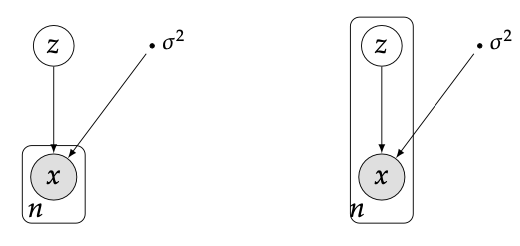
\includegraphics[width=0.9\textwidth]{assets/fig3.png}
    \end{figure}
    
\end{exampleblock}

\subsection{Sampling and reasoning in BN}

Recalling the initial example 
\[
    p(x_1,x_2,x_3,x_4) = p(x_4|x_3)p(x_3|x_2,x_1)p(x_2)p(x_1)
\]

\begin{figure}[H]
    \centering
    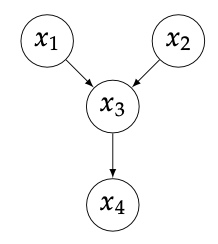
\includegraphics[width=0.2\textwidth]{assets/fig1.png}
\end{figure}

\textbf{Ancestral sampling} is a sampling technique that allows us to sample from a given distribution, if we know its factorization.

One can start to sample from the top of the network (our \textbf{ancestrals}), in the example $x_1$ and $x_2$, then move to their children and sample, in the example, $x_3$ from $p(x_3|x_2,x_1)$ using the values for $x_1$ and $x_2$ that have already been sampled, and so on. It is a simple and effective way to sample probability distribution, provided it is easy to sample from wach marginal and conditional.

\begin{exampleblock}[Reasoning with BN]
    We consider here a model of students' grade in an exam.
    \begin{figure}[H]
        \centering
        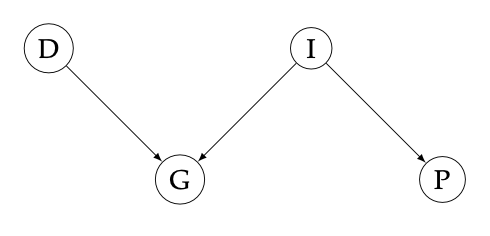
\includegraphics[width=0.7\textwidth]{assets/fig4.png}
    \end{figure}
    The difficulty of the exam (D) and the intelligence of the student (I)
    are independent, but the grade you get when you take an exam (G) is
    dependent on both (studying of course helps too). Having passed a hard
    exam (P) likely depends on the student’s abilities but not on the difficulty
    and the grade of the current exam. We have three different forms of
    reasoning here:
    \begin{itemize}
        \item \textbf{Causal Reasoning}: We observe something (the difficulty of the exams, how intelligent
        we are) and we infer the grade and if we have passed a hard exam.
        The reasoning goes from top to bottom.
        \begin{figure}[H]
            \centering
            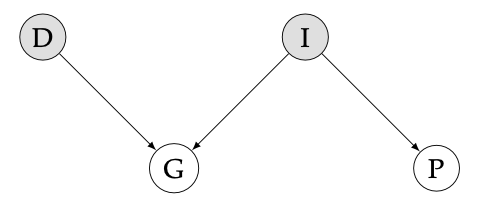
\includegraphics[width=0.7\textwidth]{assets/fig5.png}
        \end{figure}
        \item \textbf{Evidential Reasoning}: If we instead observe the grade, we might want to get information
        regarding the difficulty of the exams and how intelligent the student
        is. The reasoning goes from bottom to top.
        \begin{figure}[H]
            \centering
            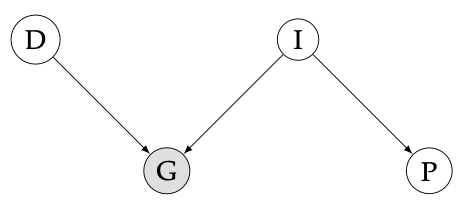
\includegraphics[width=0.7\textwidth]{assets/fig6.png}
        \end{figure}
        \item \textbf{Intercausal Reasoning}: If we observe the grade and the difficulty of the exams, we
        might want to infer the intelligence of the student. The reasoning
        goes from the middle to the top.
        \begin{figure}[H]
            \centering
            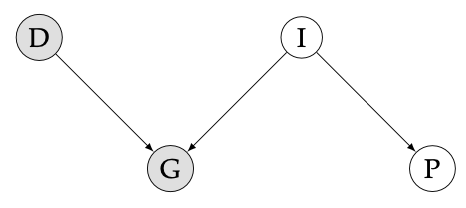
\includegraphics[width=0.7\textwidth]{assets/fig7.png}
        \end{figure}
    \end{itemize}
    Bayesian networks of course can get very large and probabilistic inference
    becomes a complicated and important task to perform in the real world.
    
    \textbf{Remark}: note that dependency in a BN can model both causality and
    correlation, and the two are not necessarily distinguishable within the
    model.
\end{exampleblock}


\newpage
\subsection{Conditional Independence in BN}

\begin{definitionblock}[Conditional Independence]
    Consider the RVs $a, b, c$. We say that $a$ is \textbf{conditional independent} of $b$ given $c$ (written $a \perp \!\!\! \perp b | c$) if:
    \[
        p(a,b|c) = p(a|c)p(b|c)
    \]
    or equivalently:
    \[
        p(a|b,c) = p(a|c)
    \]
\end{definitionblock}

We have three scenarios to consider in Bayesian Networks to understand conditional independence.

\subsubsection{Tail to Tail}

Consider the RVs $a, b, c$. We say that $a$ and $b$ are tail to tail with $c$ if:
\[
    p(a, b, c) = p(a|c)p(b|c)p(c)
\]
\begin{figure}[H]
    \centering
    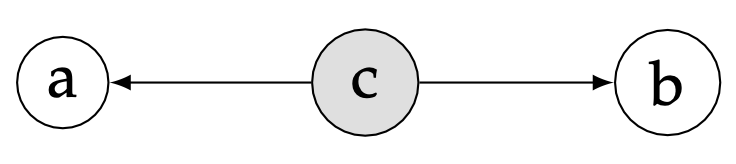
\includegraphics[width=0.5\textwidth]{assets/fig14.png}
\end{figure}

We know that this Bayesian network implies the following factorization:
\[
    p(a,b) = \sum_{c}^{}p(a|c)p(b|c)p(c) \neq p(a)p(b)
\]
Also 
\[
    p(a,b|c) = \frac{p(a,b,c)}{p(c)} = \frac{p(a|c)p(b|c)p(c)}{p(c)} = p(a|c)p(b|c)
\]
Which means that $a \perp \!\!\! \perp b \not \perp \!\!\! \perp b | c$.

\subsubsection{Head to Tail}

Consider the RVs $a, b, c$. We say that $a$ and $b$ are head to tail with $c$ if:
\[
    p(a, b, c) = p(a)p(c|a)p(b|c)
\]
or 
\[
    p(a, b, c) = p(b)p(c|b)p(a|c)
\]

\begin{figure}[H]
    \centering
    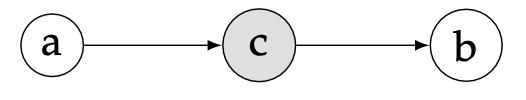
\includegraphics[width=0.5\textwidth]{assets/fig15.png}
\end{figure}

Again, we can use this factorization and study independence of our variables:
\[
    p(a,b) = \sum_{c}^{}p(a)p(c|a)p(b|c) = p(a)\sum_{c}^{}p(b|a)p(a)
\]
Also 
\[
    p(a,b|c) = \frac{p(b|c)p(c|a)p(a)}{p(c)} = p(b|c)p(a|c)
\]
Which means, again, that $a \perp \!\!\! \perp b \not \perp \!\!\! \perp b | c$.

\subsubsection{Head to Head}

Consider the RVs $a, b, c$. We say that $a$ and $b$ are head to head with $c$ if:
\[
    p(a, b, c) = p(a)p(b)p(c|a,b)
\]
\begin{figure}[H]
    \centering
    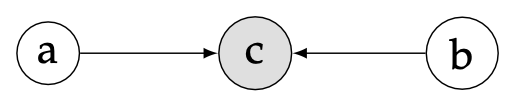
\includegraphics[width=0.5\textwidth]{assets/fig16.png}
\end{figure}

\[
    p(a,b) = \sum_{c}^{}p(a)p(b)p(c|a,b) = p(a)p(b)
\]
Also 
\[
    p(a,b|c) = \frac{p(c|a,b)p(b)p(a)}{p(c)} \neq p(b|c)p(a|c)
\]

Which means, this time, that $a \perp\!\!\!\perp b and a \not \perp\!\!\!\perp b|c$.\\
Notice that also $a \perp\!\!\!\perp b|d, \forall d$ descendant of $c$. 

\subsubsection*{Formalization}
Formalizing the notion of conditional independence on Bayesian Network that we just saw,
\begin{definitionblock}
    Given RVs $a, b, c$ $a$ path from $a$ to $b$ is \textbf{blocked} by $c$ if:
    \begin{itemize}
        \item $c$ is observed and the path is head-to-tail or tail-to-tail in $c$.
        \item $c$ is not observed, nor any descendant of $c$, and the path is head-to-head in $c$.
    \end{itemize}
\end{definitionblock}

\textbf{Proposition:} Let $A,B,C$ subsets, if all paths from a node in $A$ to a node in $B$ are blocked by a node in $C$ then $A \perp\!\!\!\perp B|C$.

\subsubsection{Markov Blanket}

Consider a node $x_i$ on the network and condition on everything else, i.e. on $x_{-i} = \{x_1, \dots, x_{i-1}, x_{i+1}, \dots, x_n\}$. Which nodes will remain in the conditioning set? If we make the computation 
\[
    p(x_i|x_{-i}) = \frac{p(x_1, \dots, x_n)}{p(x_1, \dots, x_{i-1}, x_{i+1}, \dots, x_n)} = \frac{\prod_{j}^{}p(x_j|pa_j)}{\sum_{x_i}^{}\prod_{j}^{}p(x_j|pa_j)}
\]

In the denominator, each term in which $x_i$ does not appear either as $x_j$ or in $+pa_j$ will get out of the summation and cancel with the respective term in the numerator. So the only nodes that remain are thos belonging to $pa_i$, or those for which $x_i \in pa_j$ is known as the \textbf{Markov Blanket} of $x_i$ (it contains parents, children and co-parents of $x_i$). Each node conditioned on its Markov blanket is independent of the rest of the network. 

\begin{figure}[H]
    \centering
    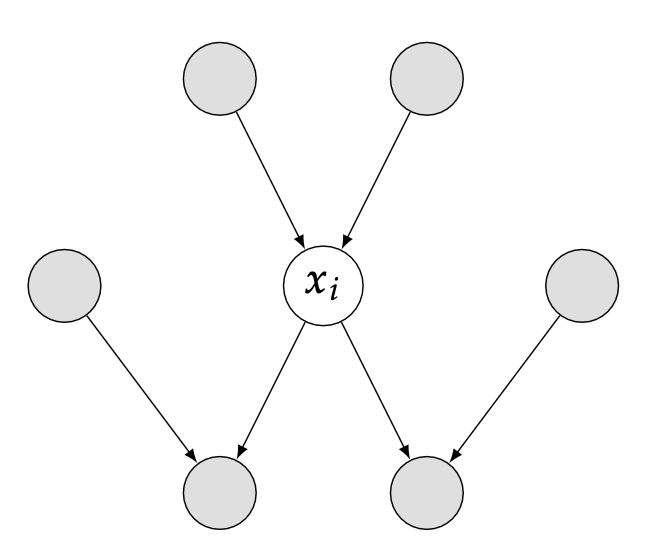
\includegraphics[width=0.5\textwidth]{assets/fig17.png}
\end{figure}

\subsection{Naive Bayes}
\begin{center}
\begin{tikzpicture}[
    roundnode/.style={circle, draw=black, minimum size=1cm},
    directed/.style={->, thick}
]

    % Nodes
    \node[roundnode] (x3) {$x_3$};
    \node[roundnode, above left=1cm and 1cm of x3] (x1) {$x_1$};
    \node[roundnode, above right=1cm and 1cm of x3] (x2) {$x_2$};
    \node[roundnode, below=1.5cm of x3] (x4) {$x_4$};

    % Arrows
    \draw[directed] (x1) -> (x3);
    \draw[directed] (x2) -> (x3);
    \draw[directed] (x3) -> (x4);

\end{tikzpicture}
\end{center}